\section{Bi-continuous and non-particular structures}
\subsection{TeubnerStrey}
\label{sect:TeubnerStrey}~\\

The Teubner and Strey \cite{TeubnerStrey87,StreyKlineKaler1994}
phenomenological model often accurately describes scattering from
bi-continuous micro-emulsions. The scattered intensity for this
model is
\begin{align}
I(q) = \frac{8\pi\langle\eta^2\rangle/\xi}{a^2-2bq^2+q^4}
\end{align}
where $a^2=(k^2+1/\xi^2)^2$ is a positive quantity, and
$b=k^2-1/\xi^2$ can be a positive or negative depending on the
relative magnitude of $d=2\pi/k$ and $\xi$. A positive $b$, i.e.
$\xi>d/2\pi$, leads to a peak at $q_\text{max}=\sqrt{b}$ whereby for
$\xi<d/2\pi$, hence negative $b$, no distinct peak appears. The
length scale $d$ represents a quasi-periodic repeat distance between
water and oil regions within the solution, while the correlation
length, $\xi$ , corresponds to a characteristic length for
positional correlation. $k$ is defined as $2\pi/d$. The
corresponding isotropic real space correlation function,
$\gamma(r)$, that incorporates alternating regions of the two phases
in the bi-continuous system (e.g. water and oil), is given by
\begin{align}
\gamma(r) = \frac{\sin(kr)}{kr} \exp\left(-\frac{r}{\xi} \right)
\end{align}

\vspace{5mm}

\underline{Input Parameters for model \texttt{TeubnerStrey}:}\\
\begin{description}
\item[\texttt{xi}] correlation length $\xi$
\item[\texttt{d}] characteristic domain size $d$
\item[\texttt{eta2}] squared scattering length density contrast $\eta^2$
\end{description}

\underline{Note:}
\begin{itemize}
\item None
\end{itemize}


\begin{figure}[htb]
\begin{center}
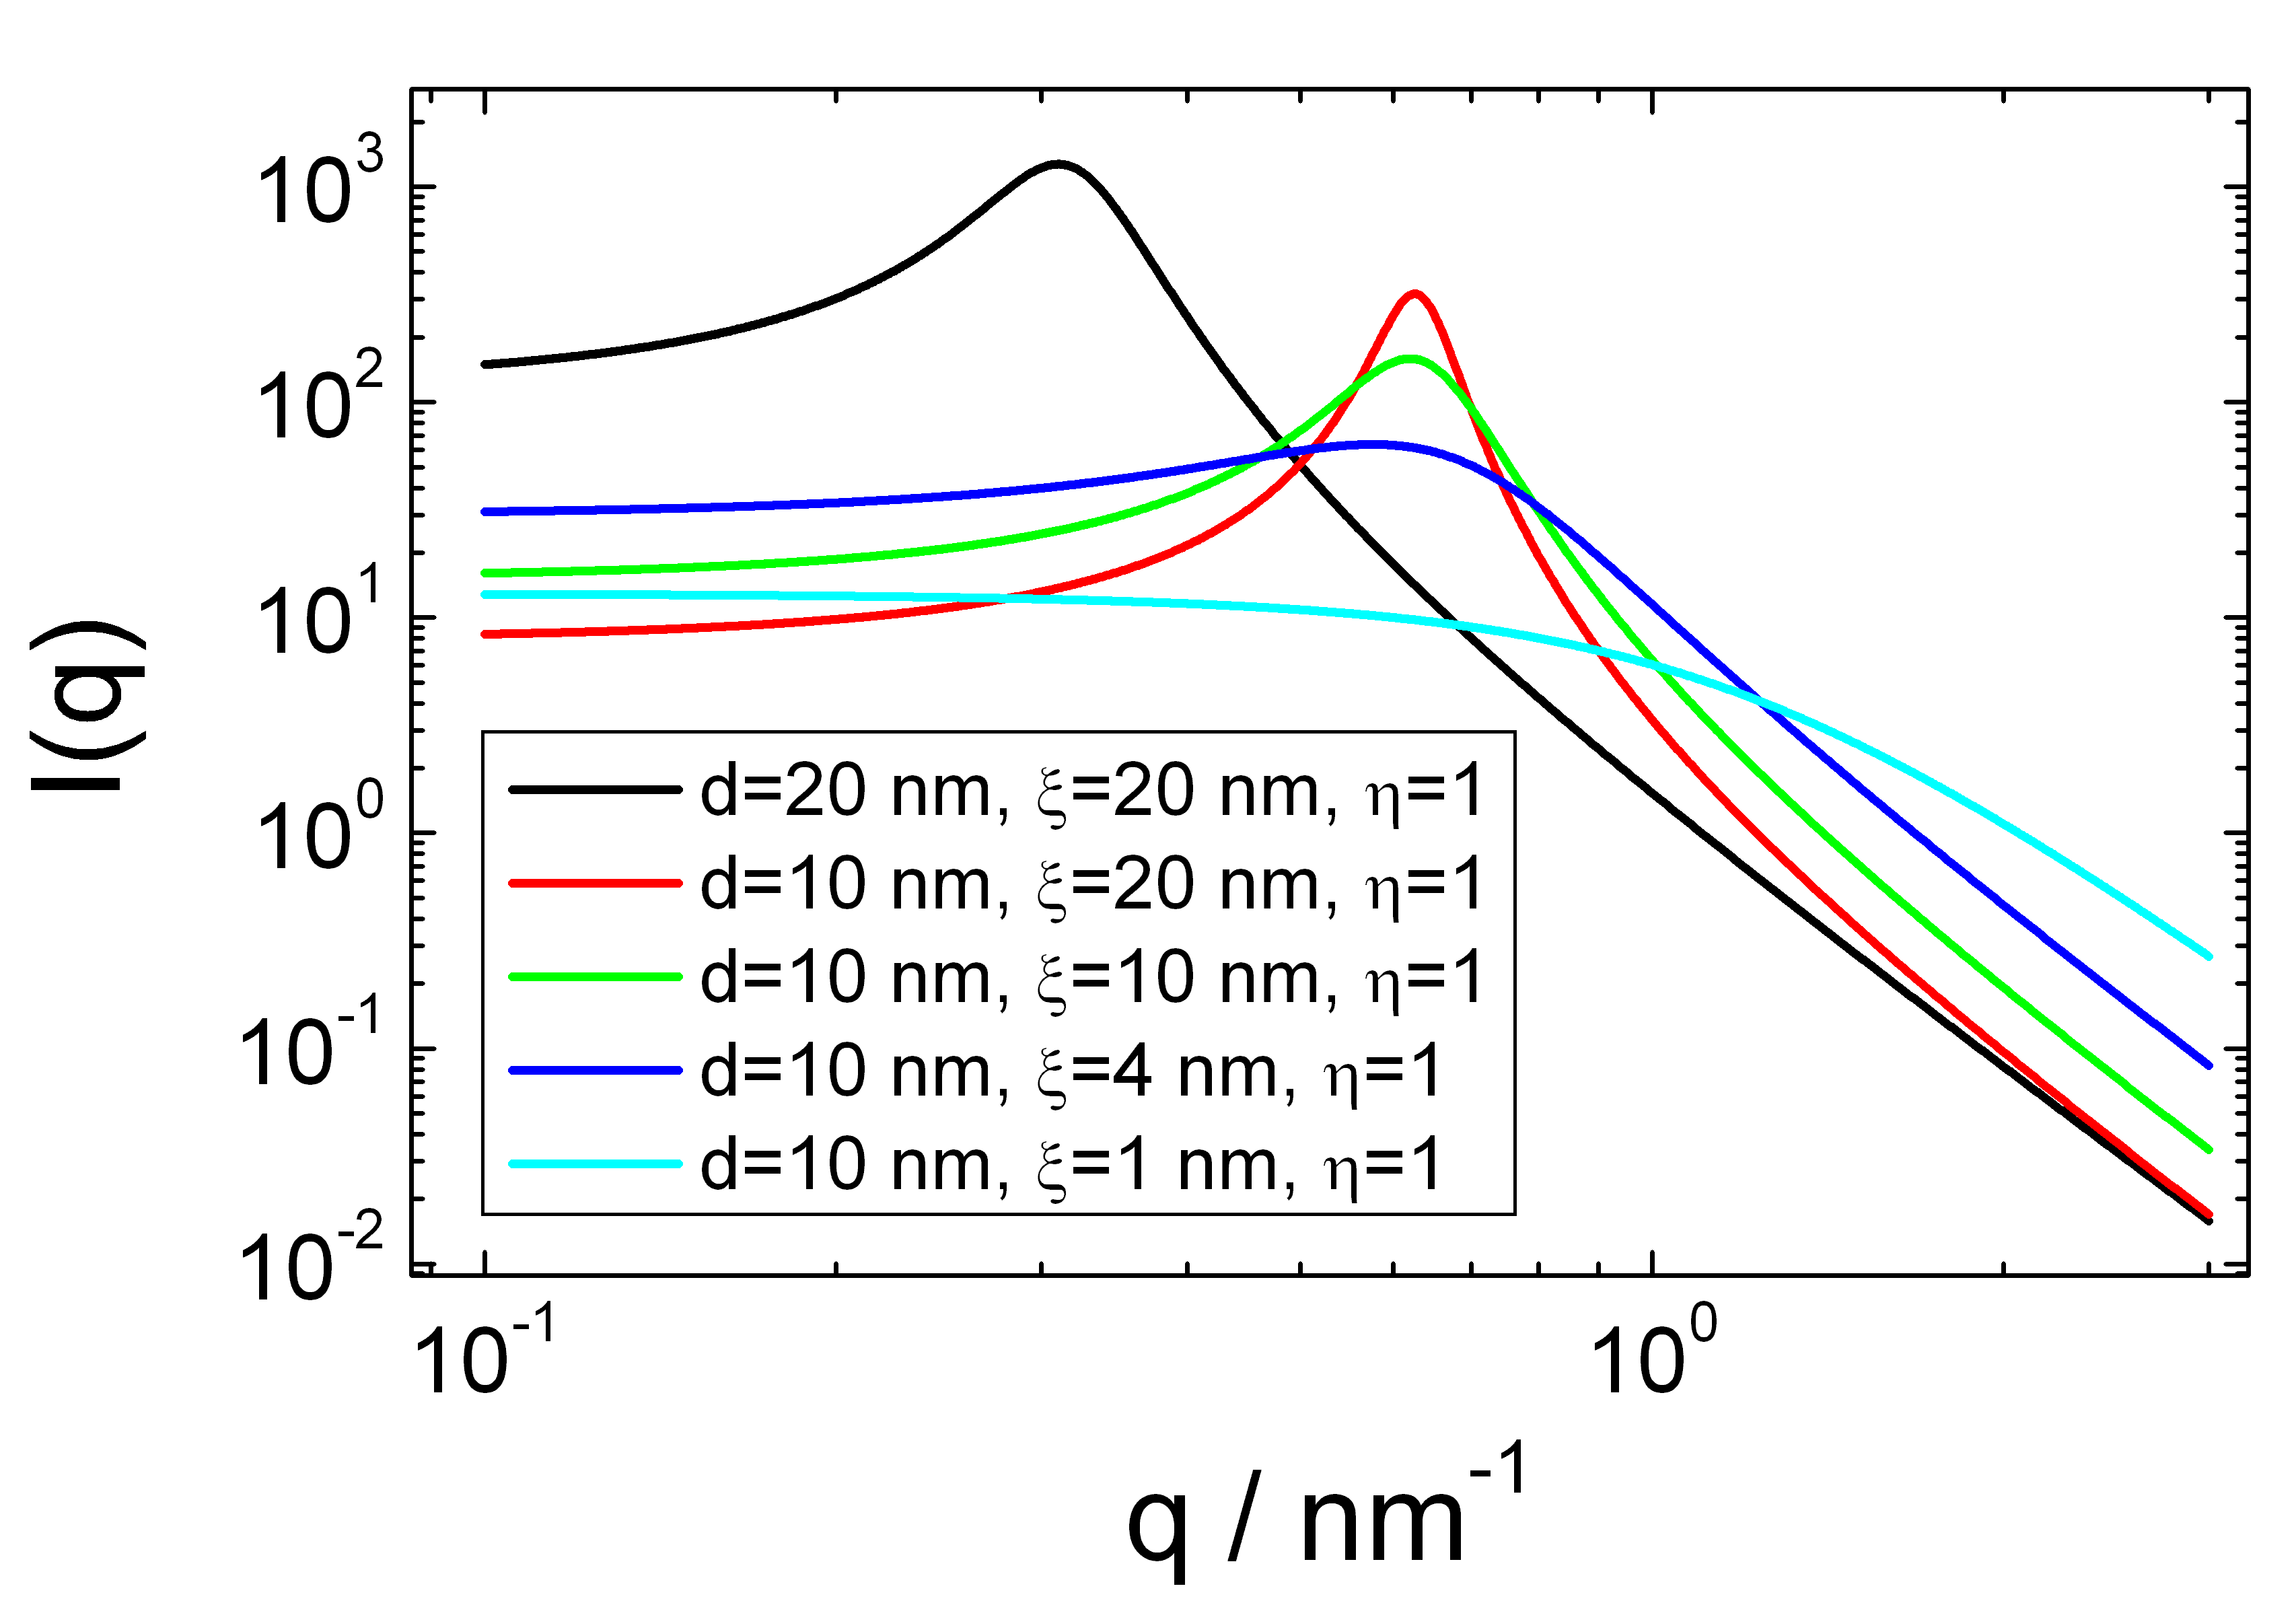
\includegraphics[width=0.85\textwidth,height=0.6\textwidth]{TeubnerStrey.png}
\end{center}
\caption{} \label{fig:TeubnerStreyIq}
\end{figure}
%\vspace{5mm}
%\noindent REFERENCE:\\
%Teubner, M; Strey, R. J. Chem. Phys., 1987, 87, 3195.\\
%Schubert, K-V.; Strey, R.; Kline, S. R.; and E. W. Kaler J. Chem. Phys., 1994, 101, 5343.

%%%%%%%%%%%%%%%%%%%%%%%%%%%%%%%%%%%%%%%%%%%%%%%%%%%%%%%%%%%%%%%%%%%%%%%%%

\clearpage
\subsection{Debye Anderson Brumberger(DAB)}
\label{sect:DAB}~\\

This form factor calculates the scattering from a randomly
distributed (i.e. non-particulate), two-phase system based on the
Debye-Anderson-Brumberger (DAB) \cite{DAB1957,DebyeBueche1949} model
for such systems. The two-phase system is characterized by a single
length scale, the correlation length $\xi$, which is a measure of
the average spacing between regions of phase 1 and phase 2. The
model also assumes smooth interfaces between the phases and hence
exhibits Porod behavior ($I \propto q^{-4}$) at large $q$ ($q \xi
\gg 1$). The pair correlation function is give by
\cite{DebyeBueche1949}
\begin{align}
\gamma(r) = \exp(-r/\xi)
\end{align}
The macroscopic scattering cross-section in the DBA model is given
by
\begin{align}
I(q) = I_0 \frac{1}{\left[1+(q\xi)^2\right]^2}
\end{align}


\underline{Input Parameters for model \texttt{DAB}:}\\
\begin{description}
\item[\texttt{xi}] correlation length $\xi$
\item[\texttt{I0}] forward scattering $I_0$
\end{description}

\underline{Note:}
\begin{itemize}
\item None
\end{itemize}


\begin{figure}[htb]
\begin{center}
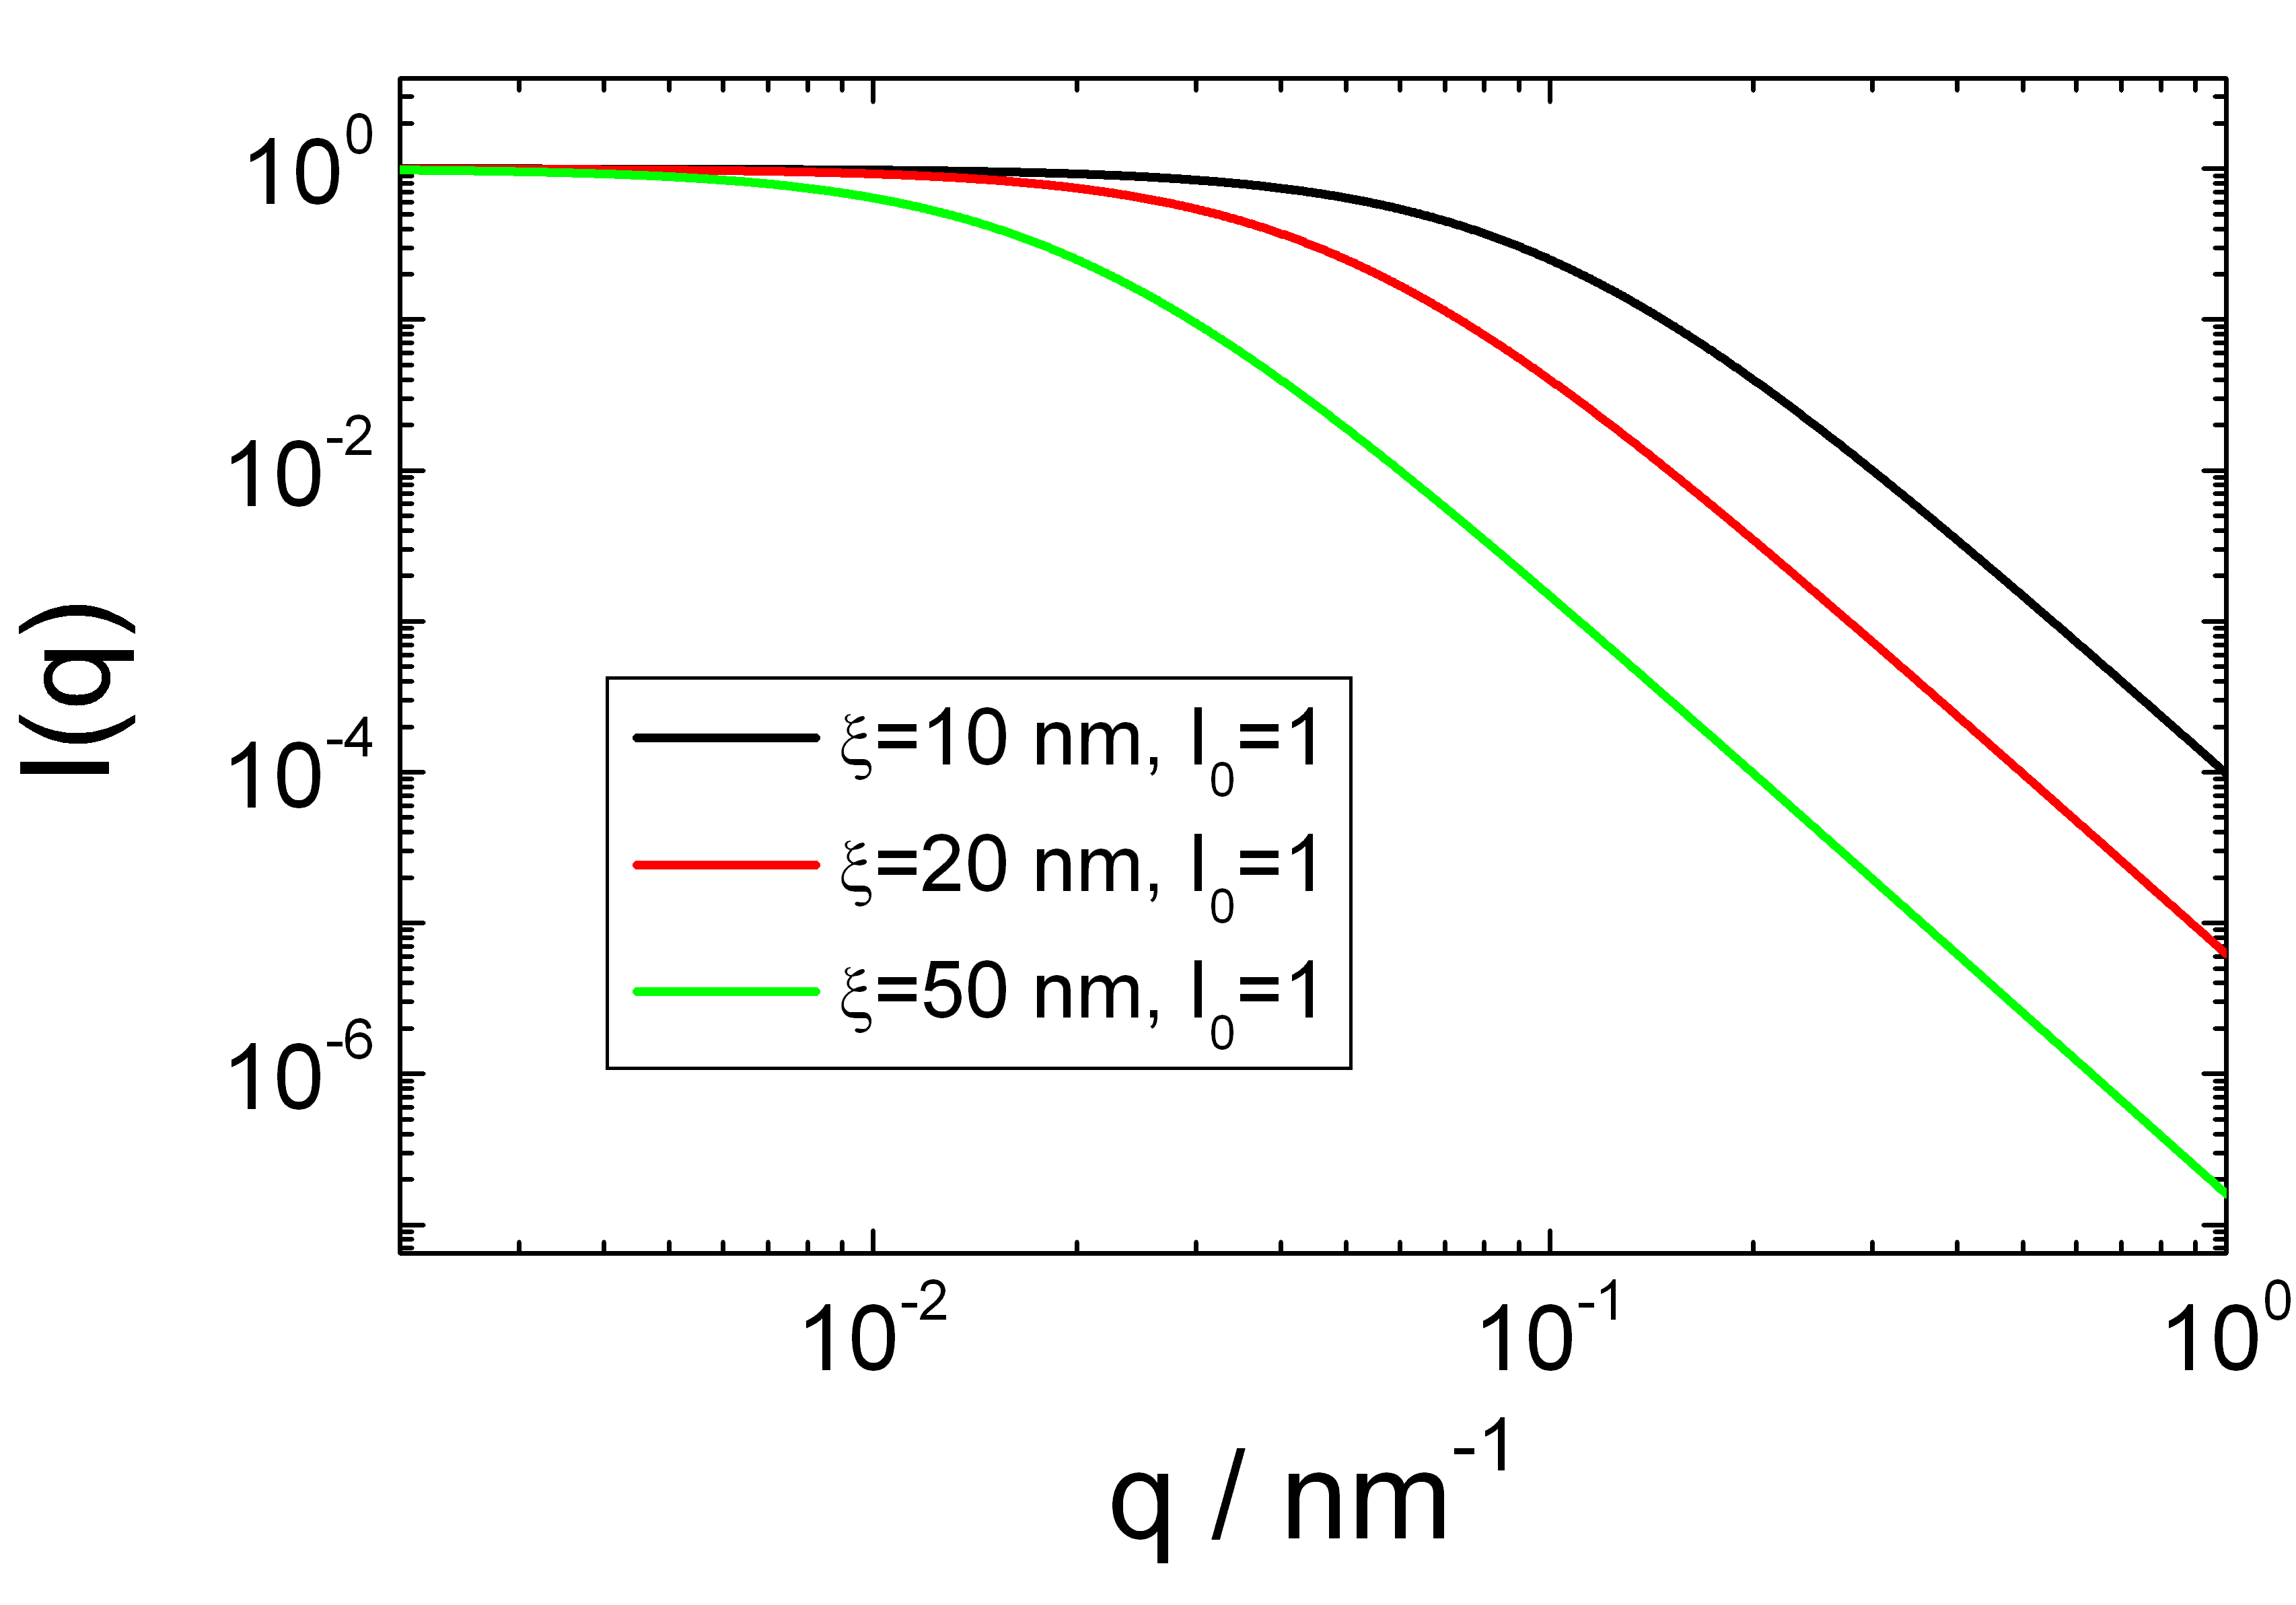
\includegraphics[width=0.85\textwidth,height=0.6\textwidth]{DAB.png}
\end{center}
\caption{} \label{fig:DABIq}
\end{figure}


%%%%%%%%%%%%%%%%%%%%%%%%%%%%%%%%%%%%%%%%%%%%%%%%%%%%%%%%%%%%%%%%%%%%%%%%%

\clearpage
\subsection{Spinodal}
\label{sect:Spinodal}
~\\

\begin{figure}[htb]
\begin{center}
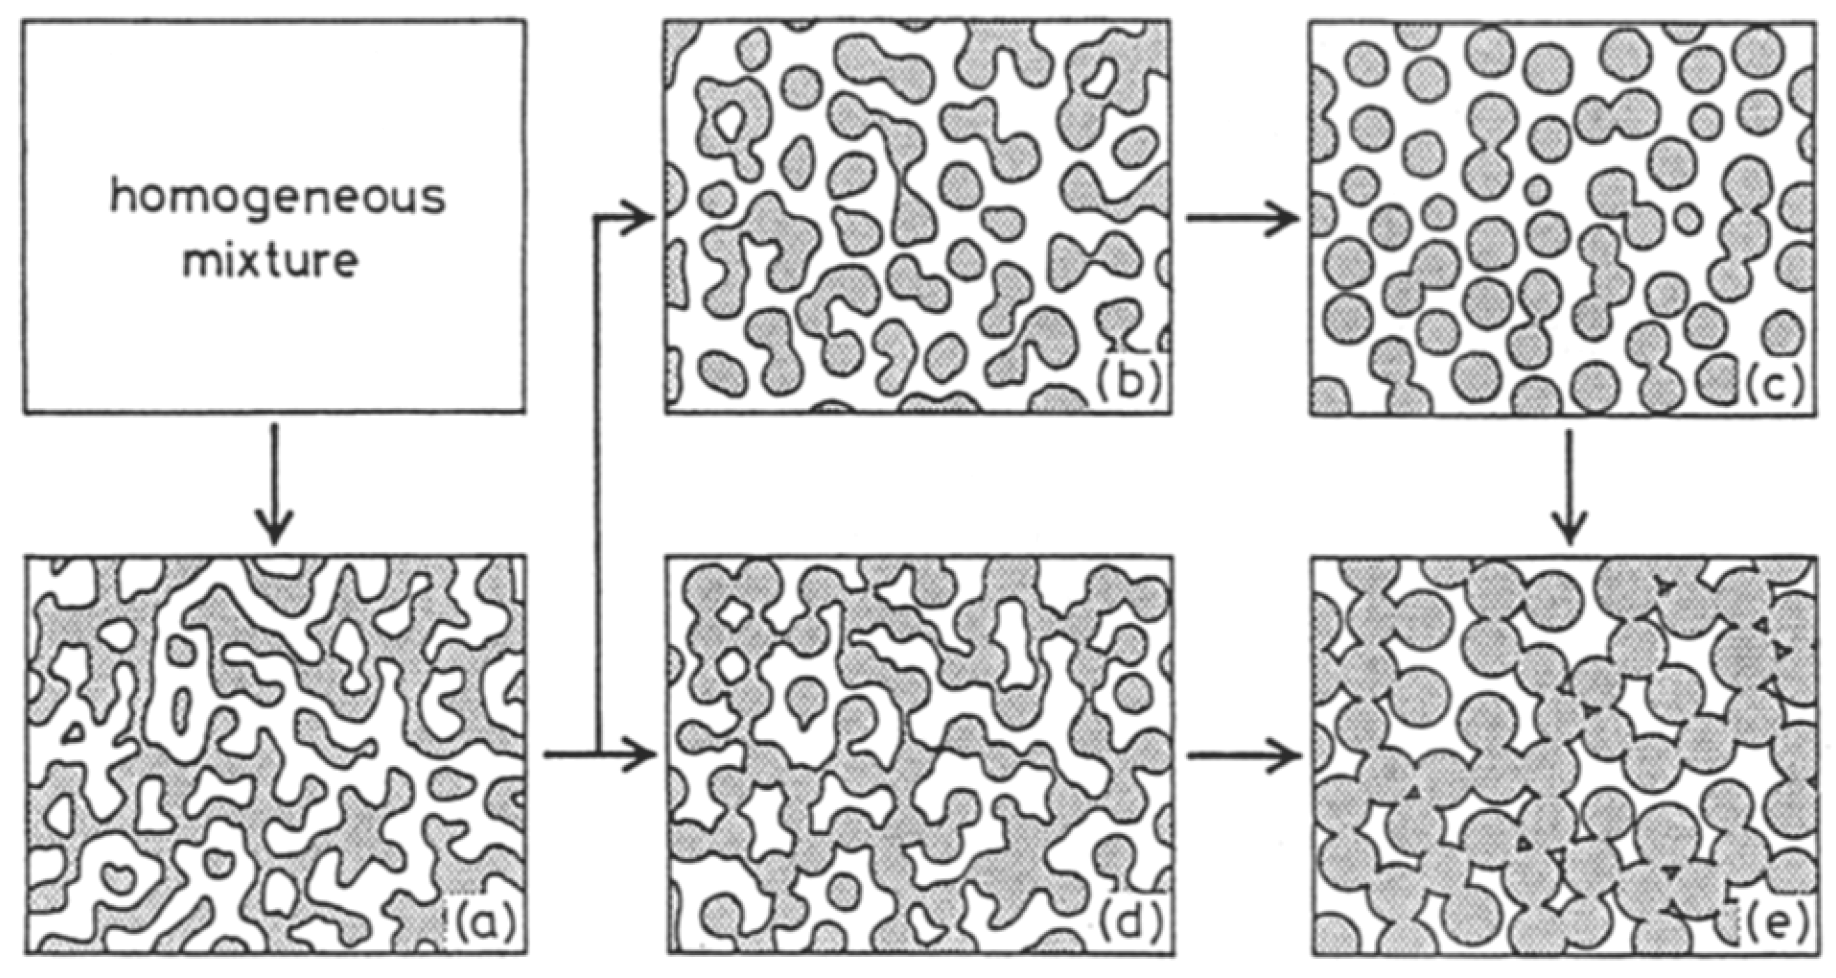
\includegraphics[width=0.648\textwidth,height=0.345\textwidth]{spinodal2.png}
\end{center}
\caption{Schematic representation of a phase separation scheme
resulting in a connected globule structure.} \label{Spinodal}
\end{figure}

Spinodal decomposing systems show a characteristic small angle
scattering signal with a correlation peak at some scattering value
$q_\text{max}$. The scattering curve $I(q)$ can be approximated by
\begin{align}
I(q) = I_\text{max} \frac{(1+\gamma/2)x^2}{\gamma/2+x^{2+\gamma}}
\end{align}
according to Furukawa \cite{Furukawa1984}, where $x=q/q_\text{max}$.
The position of the correlation peak at $q_\text{max}$ contain
information about the size of the structures, which scatter. The
exponent $\gamma$ is equal to $\gamma=D+1$ for off-critical mixtures
and $\gamma=2D$ for critical concentration mixtures, whereby $D$ is
the dimensionality of the system.

\vspace{5mm}

\underline{Input Parameters for model \texttt{Spinodal}:}\\
\begin{description}
\item[\texttt{Qmax}] peak maximum $q_\text{max}$
\item[\texttt{gamma}] exponent $\gamma$
\item[\texttt{Imax}] scattering intensity at peak position $I_\text{max}$
\end{description}

\underline{Note:}
\begin{itemize}
\item None
\end{itemize}



\begin{figure}[htb]
\begin{center}
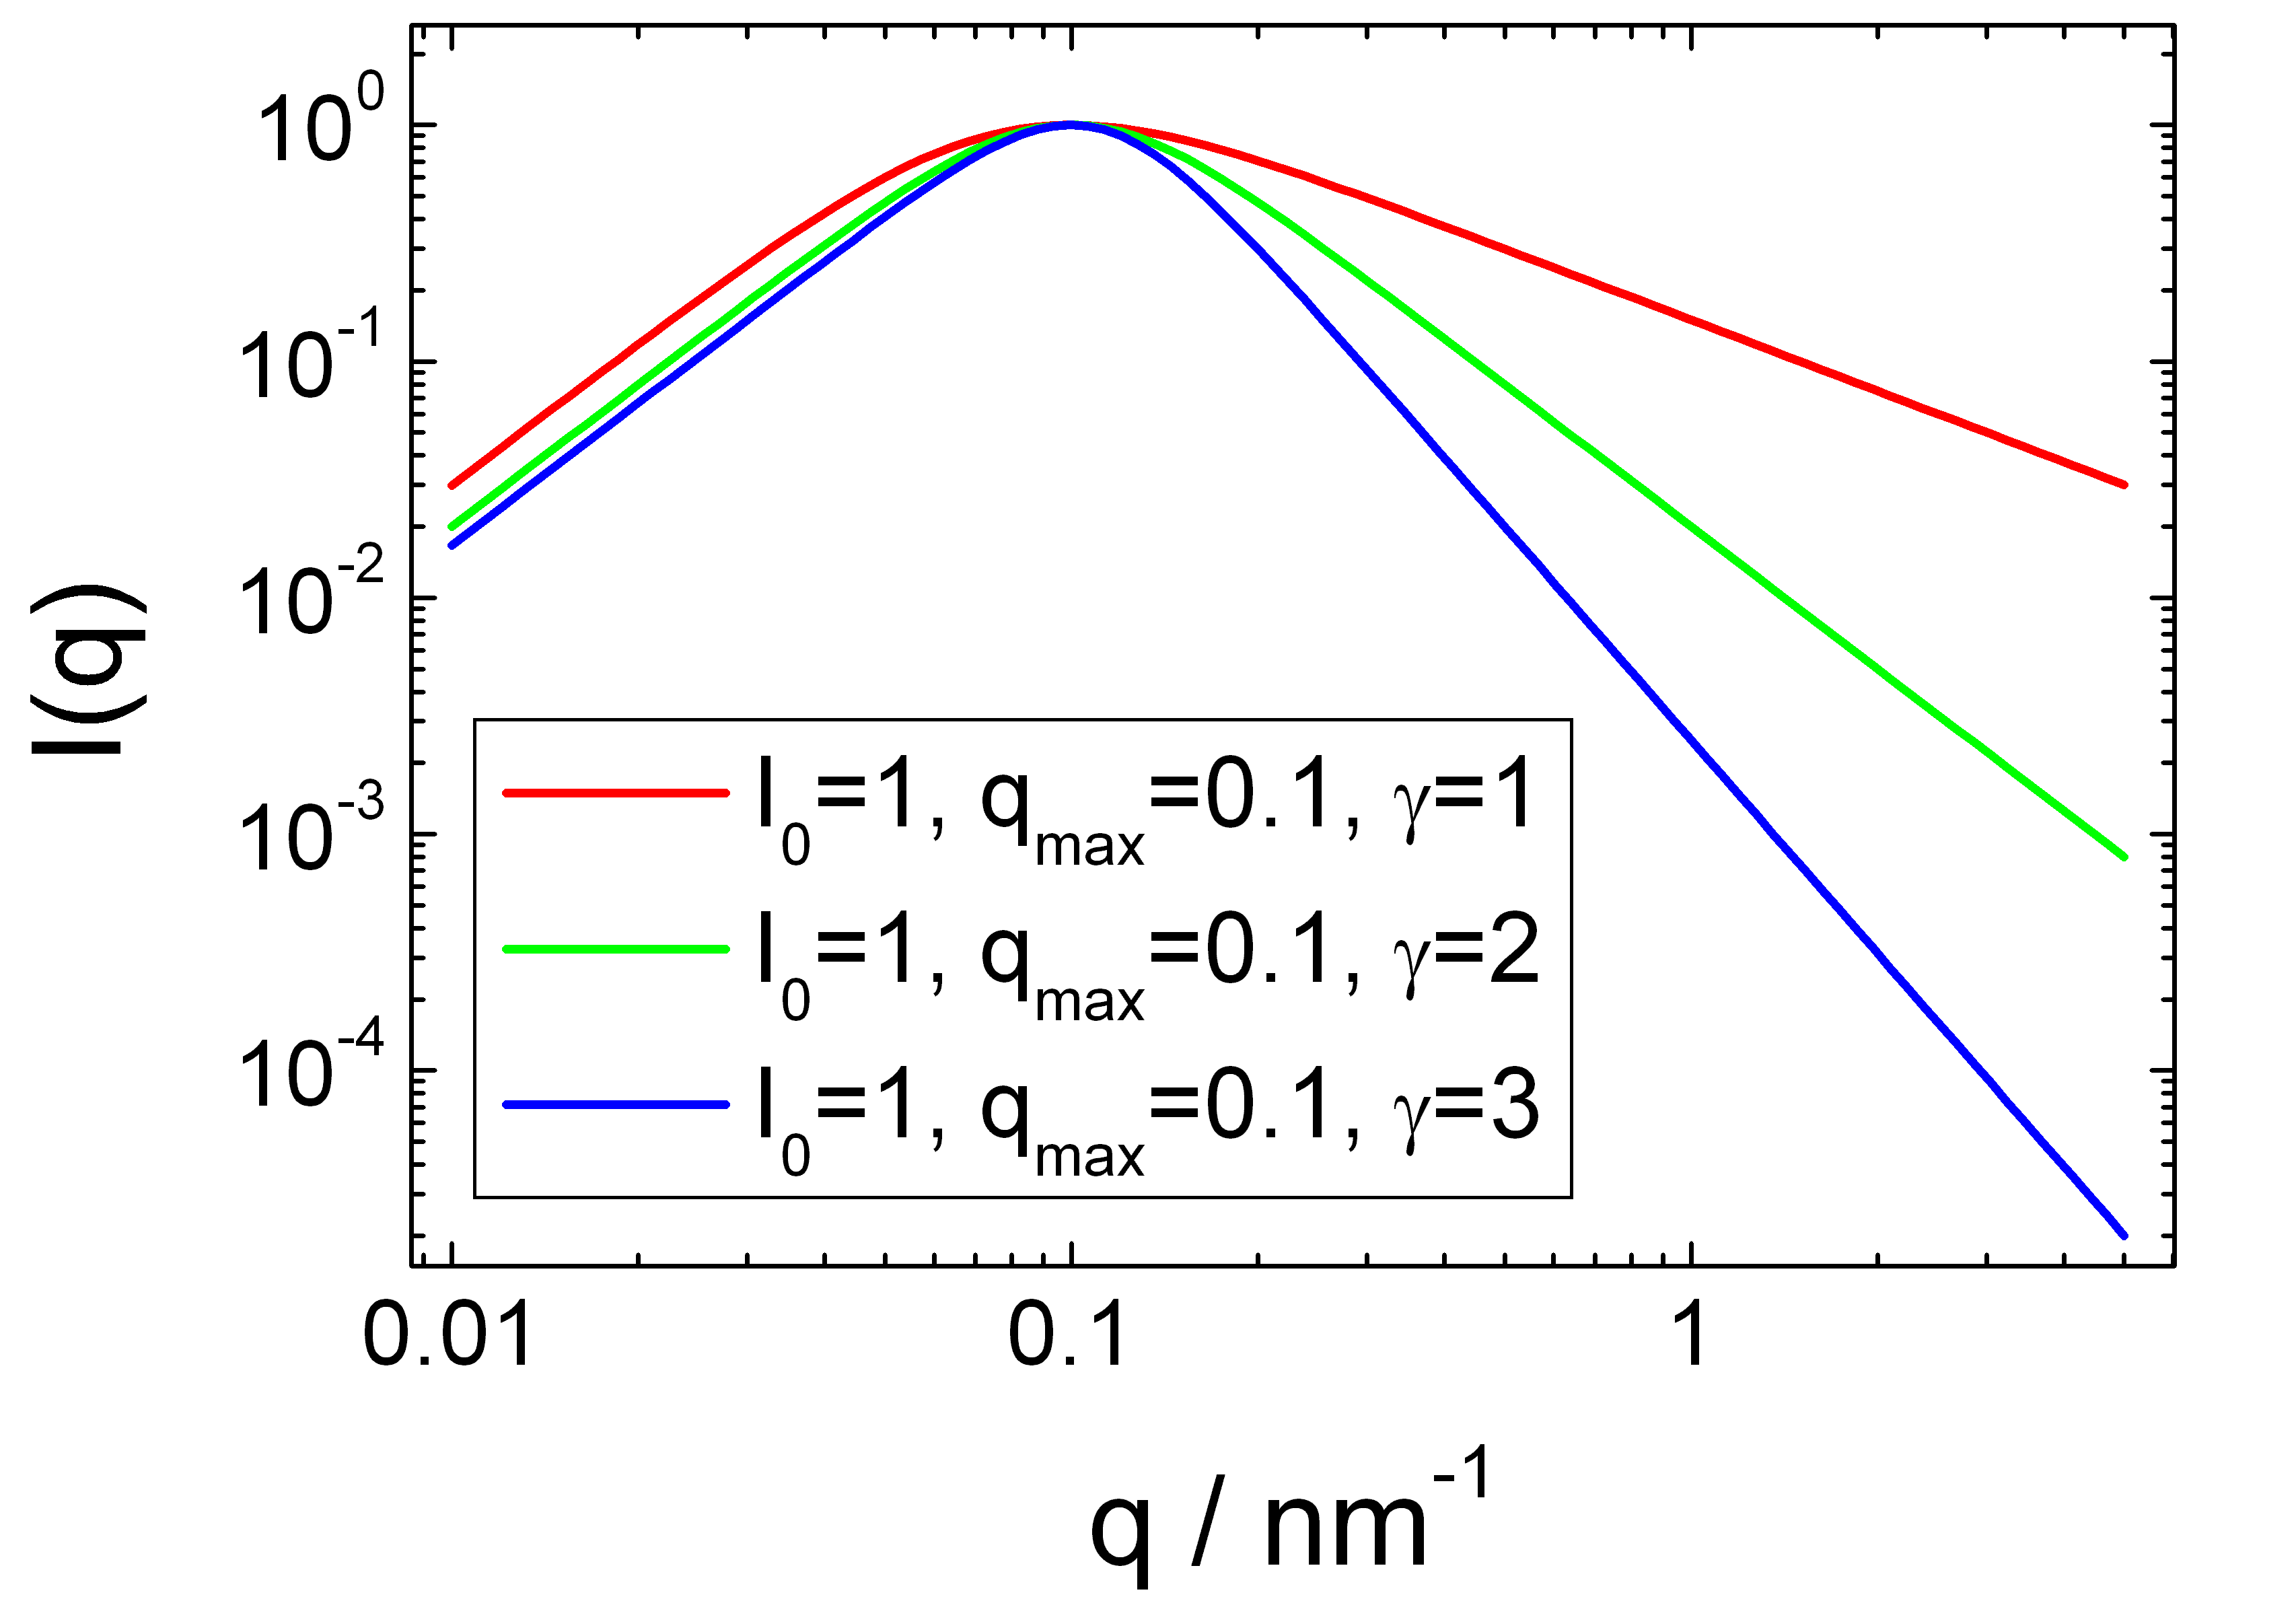
\includegraphics[width=0.85\textwidth,height=0.6\textwidth]{spinodalIQ.png}
\end{center}
\caption{} \label{fig:spinodalIQ}
\end{figure}

\clearpage
\subsection{OrnsteinZernike}
\label{sect:Zernike}
 ~\\
The low-angle scattering of thermal composition fluctuations can be
described according to the Ornstein-Zernike formulation by a
Lorentzian profile
\begin{align}
I(q) = \frac{I_0}{1+q^2\xi^2}
\end{align}
characterizing the exponential decay of the composition fluctuations
correlation function, with correlation length $\xi$. The Fourier
transform of a Lorentzian function corresponds to correlations dying
out as $\gamma(r) \simeq \frac{1}{r}exp(-r/\xi)$. Note that the
low-$Q$ limit of this empirical form reproduces the Guinier law.

\hspace{1pt}\\
\underline{Input Parameters for model \texttt{OrnsteinZernike}:}\\
\begin{description}
\item[\texttt{I0}] forward scattering $I_0$ at $q=0$.
\item[\texttt{xi}] correlation length $\xi$
\end{description}

\begin{figure}[htb]
\begin{center}
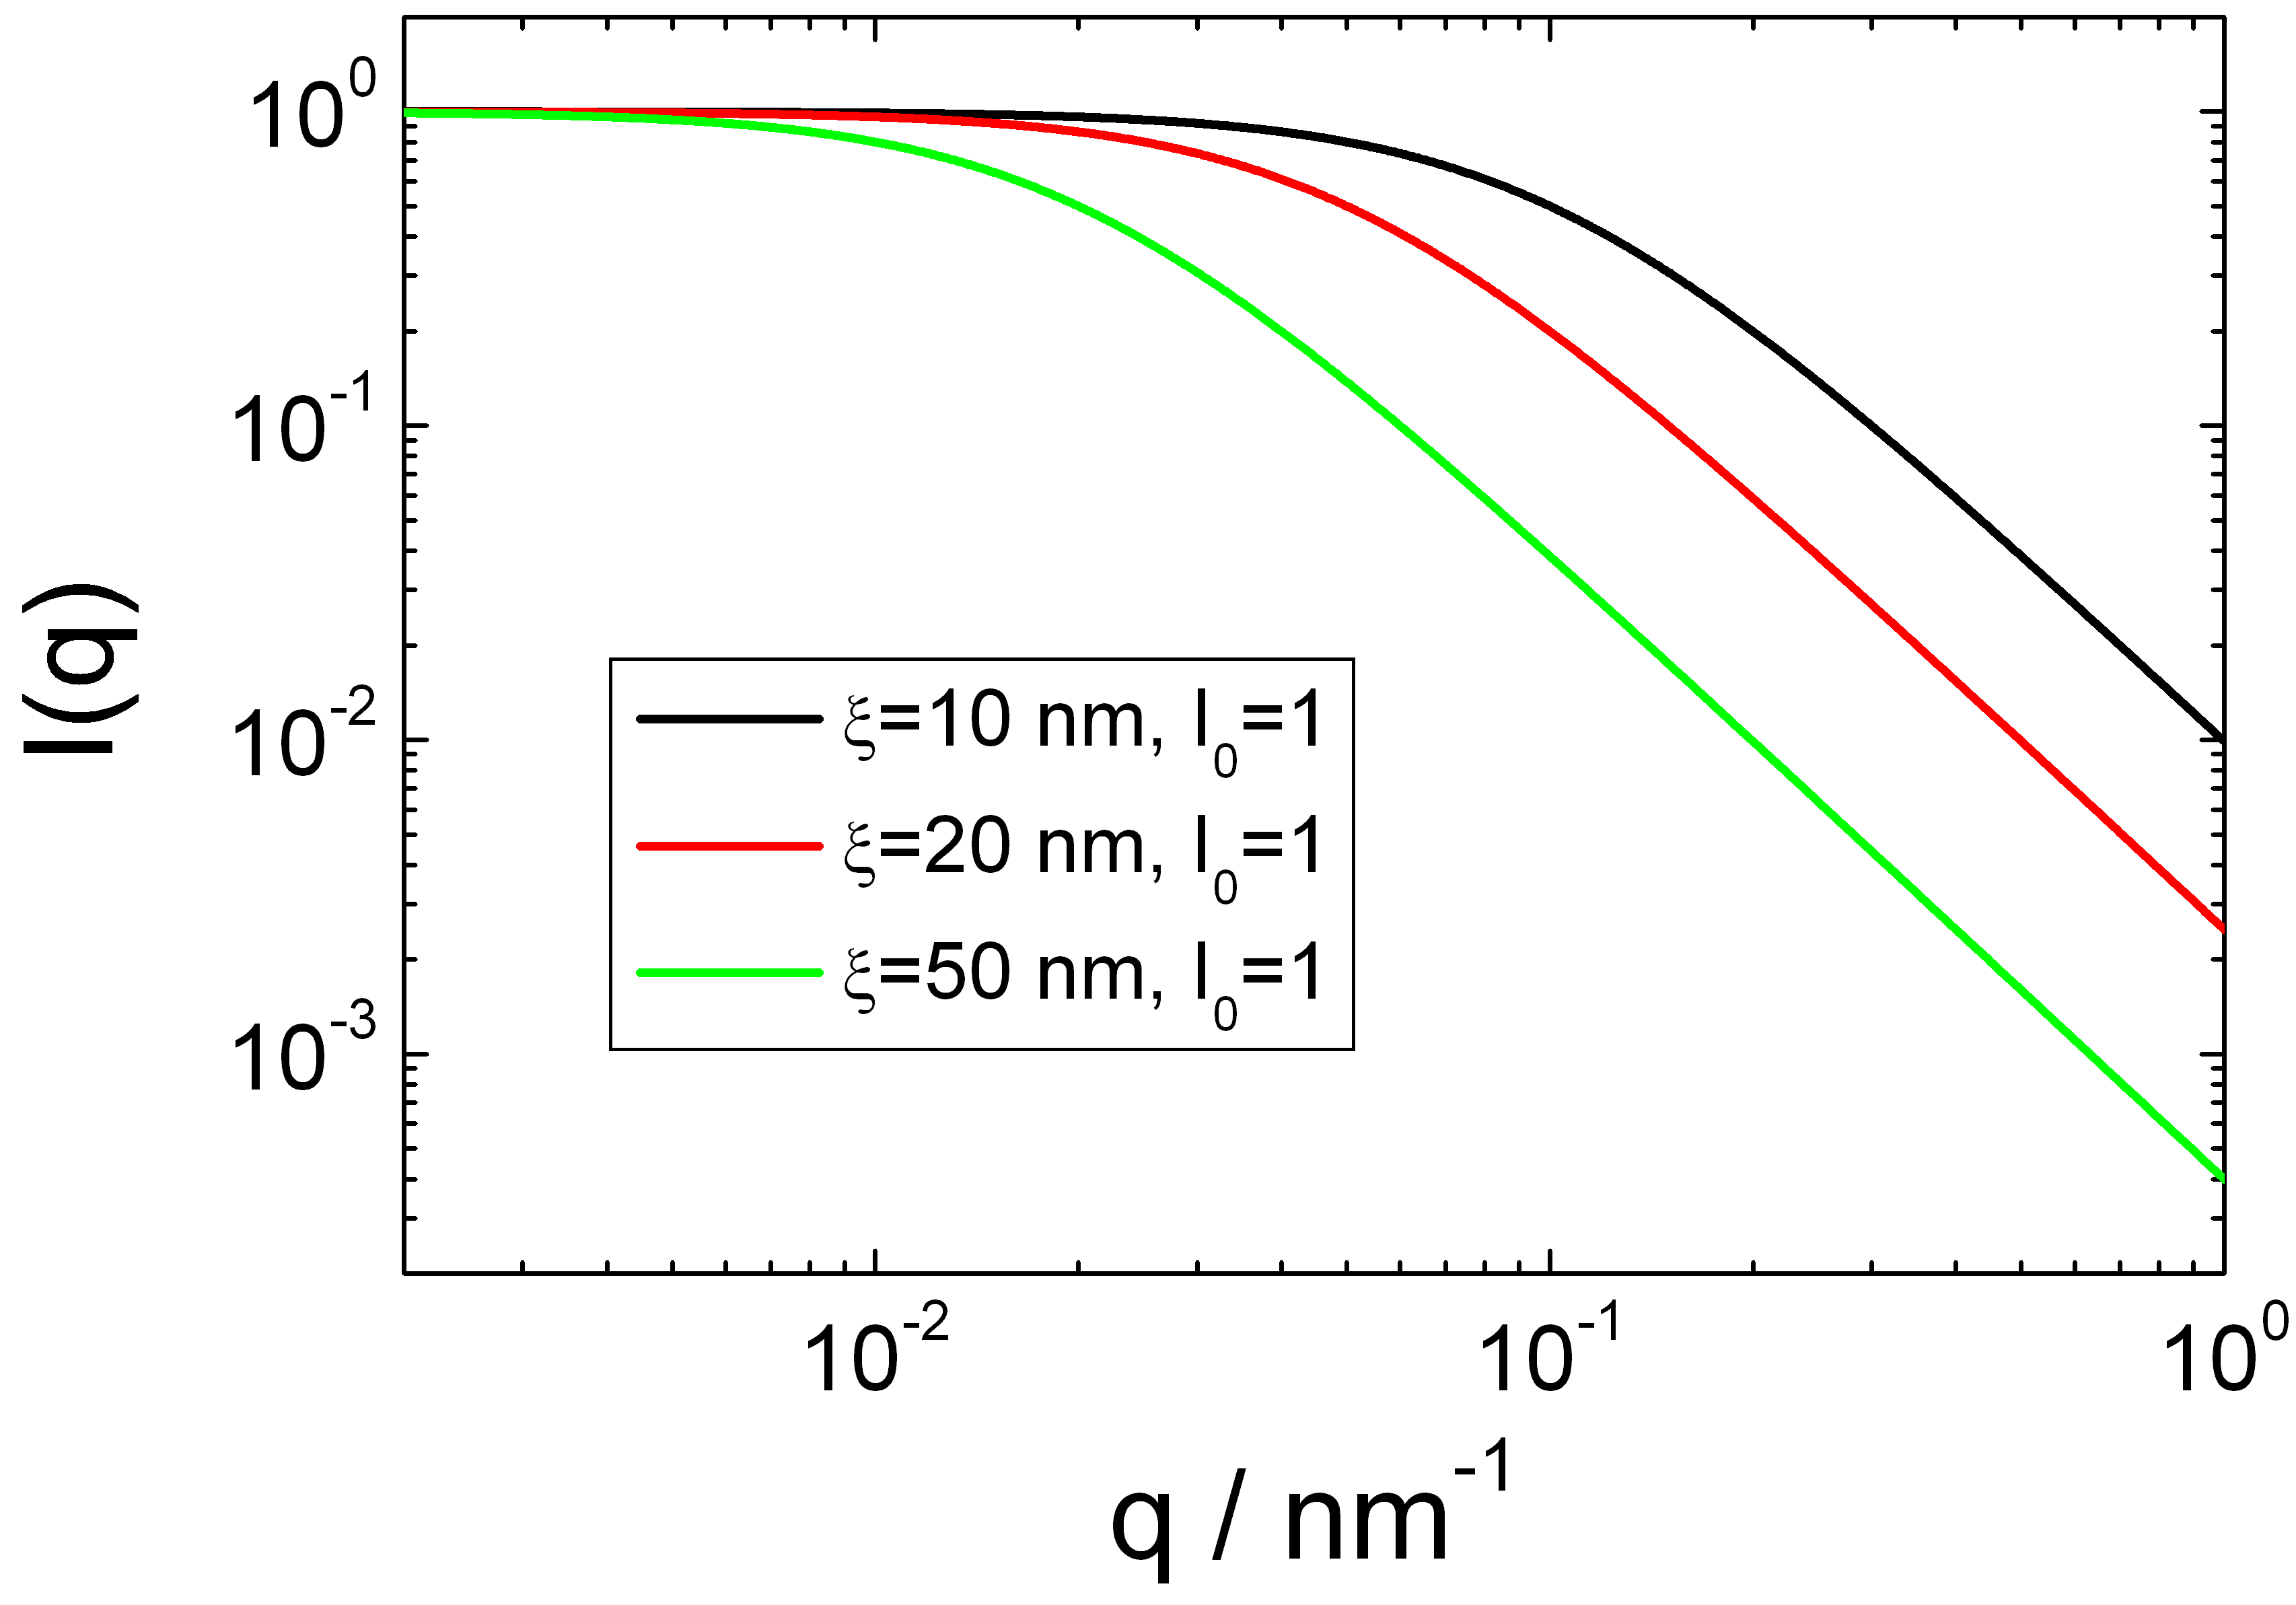
\includegraphics[width=0.85\textwidth,height=0.6\textwidth]{OrnsteinZernicke.png}
\end{center}
\caption{Ornstein-Zernike Scattering intensity $I(q)$ for different
correlation lengths $\xi$} \label{fig:OrnsteinZernicke}
\end{figure}
\clearpage

\subsection{BroadPeak}
\label{sect:BroadPeak}
 ~\\
Many SANS spectra are characterized by a broad peak even though they
are from amorphous soft materials. The $d$-spacing corresponding to
the broad peak is a characteristic distance between the scattering
inhomogeneities (such as in lamellar, cylindrical, or spherical
morphologies or for bicontinuous structures). The following simple
functional form reproduces the broad peak feature:
\begin{align}
I(q) = \frac{I_0}{1+\left(\abs{q-q_0}\xi\right)^m}
\end{align}
Here the peak position is related to the $d$-spacing as $q_0 =
2\pi/d$. Soft systems that show a SANS peak include copolymers,
polyelectrolytes, multiphase systems, layered structures, etc.


\clearpage
\subsection{Generalized Guinier approximation \cite{Fratzl1994,Hjelm1992,Hjelm1995,Hjelm2000}}
\label{sec:generalizedGuinier}  ~\\

\begin{figure}[htb]
\begin{center}
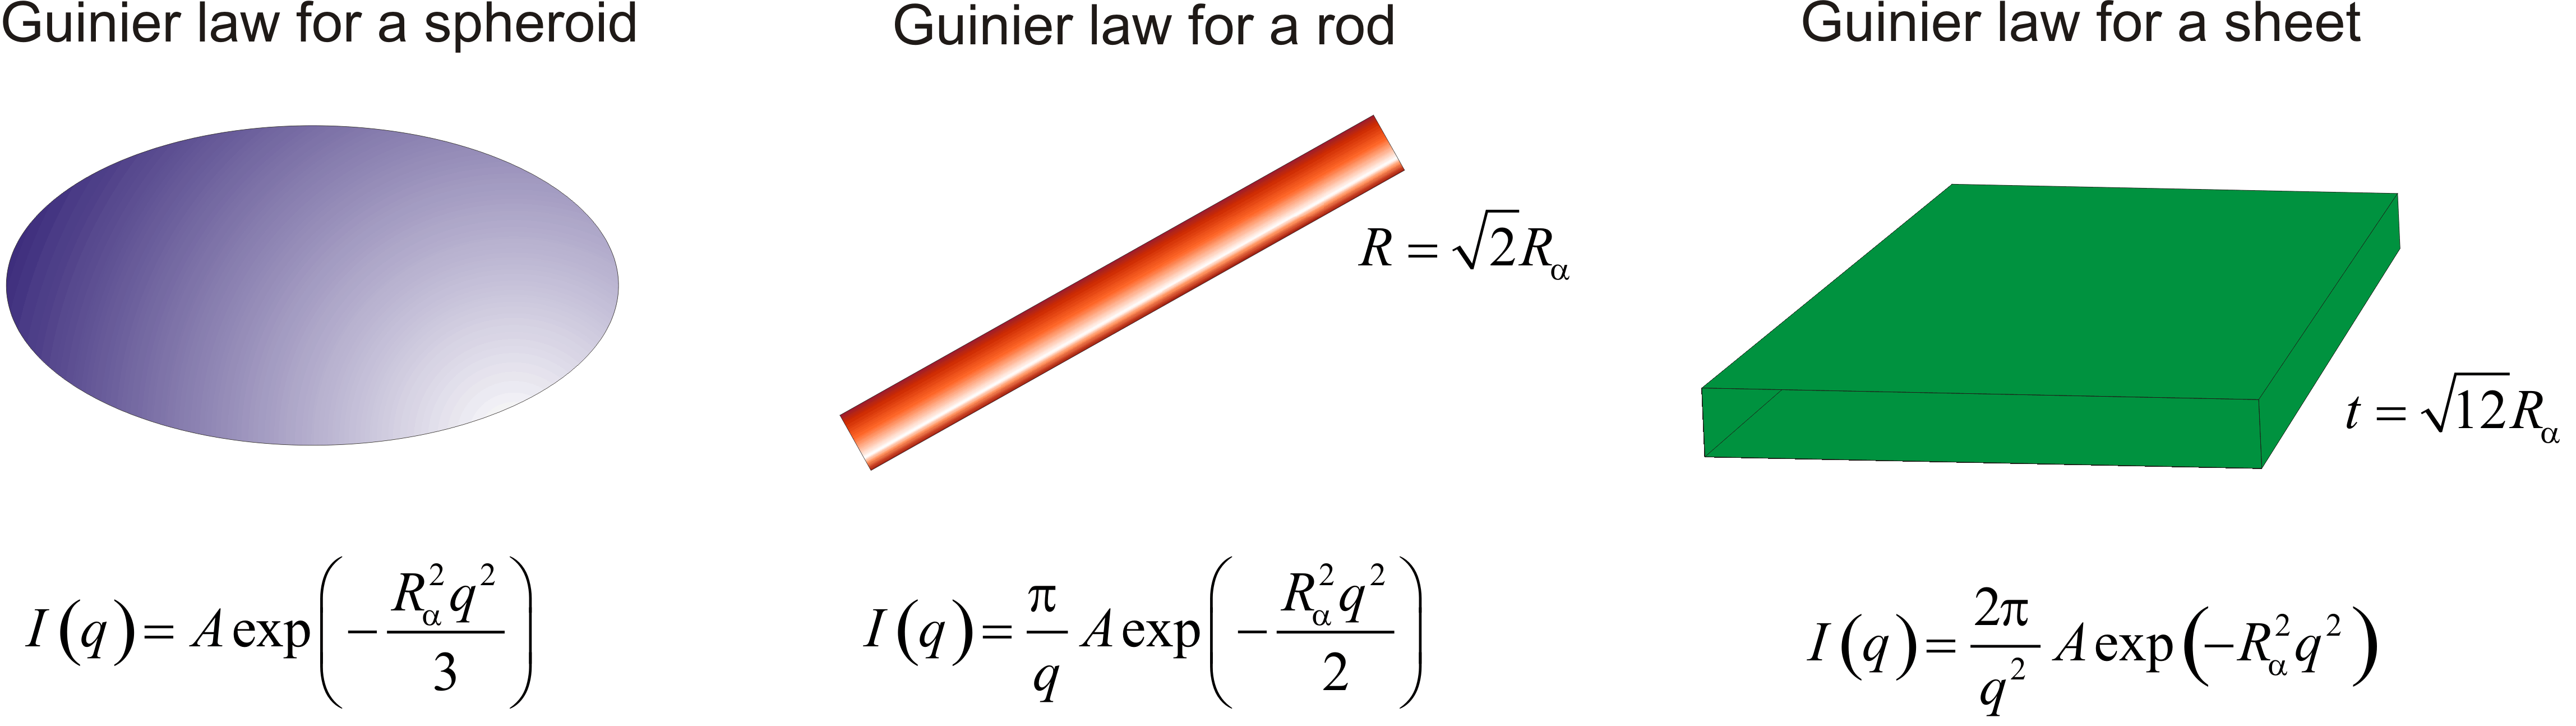
\includegraphics[width=0.75\textwidth,height=0.25\textwidth]{generalizedGuinier_q.png}
\end{center}
\caption{generalized Guinier approximation}
\end{figure}
Quantitative analysis of particle size and shape starts with the
Guinier approximations. For three-dimensional objects the Guinier
approximation is given by $I(q) = \exp(-Rg^2q^2/3)$ This
approximation can be extended also to rod-like and plane objects by
\begin{align}
I(q) &= \left\{
\begin{array}{lll}
  1 & \mbox{for} & \alpha=0 \\
  \alpha \pi q^{-\alpha} & \mbox{for} & \alpha=1,2 \\
\end{array}
\right\} A \,\, \exp\left(-\frac{R_\alpha^2 q^2}{3-\alpha}\right)
\label{eq:generalizedGuinier}
\end{align}
\begin{description}
\item[$\alpha=0$] spheroid
\item[$\alpha=1$] rod-like
\item[$\alpha=2$] plane
\end{description}
The apparent particle shape (also called the dimensionality) is
represented in eq.\ \ref{eq:generalizedGuinier} by $\alpha$, which
has integer values of 0, 1, and 2 for a point, a line, and a plane,
respectively. Equation \ref{eq:generalizedGuinier} states that there
are $q$ ranges, corresponding to length scales as $q^{-1}$, from
which the particle dimension or shape, $\alpha$, the radius of
gyration, $R_\alpha$, and the pre-factor, $A$, characteristic of
$\alpha$ can be inferred. $\alpha$ has a value of 0 for a $q$ range
such that $qR_g < 1-1.3$ (the larger applies when the particle is
known to be a spheroid), where $R_g$ is the particle radius of
gyration (computed about the particle centroid). In this case, the
pre-factor $A$ describes the excess differential cross-section per
unit mass (cm$^2$ g$^{-1}$) of a particle. If the particle has one
dimension of length $L$, that is, much larger than the others (i.e.,
elongated, rod-like, or worm-like), then there is a $q$ range such
that $qR_c < 1 \ll qL$, where $\alpha = 1$. Here, $R_c$ is the
radius of gyration (computed about a line centered along $L$) of the
cross-section perpendicular to $L$. If these conditions apply, the
pre-factor $A$ describes the excess differential cross section per
unit length per unit mass (cm$^2$ \AA$^{-1}$ g$^{-1}$). Finally, for
planar shapes, including single bilayer vesicles, with two locally
large dimensions, $D$, and planar cross-sectional radius of gyration
(computed about a central plain),$R_d$, there may be a region of $q$
such that $qR_d < 1 \ll qD$, where $\alpha = 2$. For such planar
structures, the pre-factor is the excess differential cross-section
per unit area per unit mass (cm$^2$ \AA$^{-2}$ g$^{-1}$) of a sheet.

\begin{figure}[htb]
\begin{center}
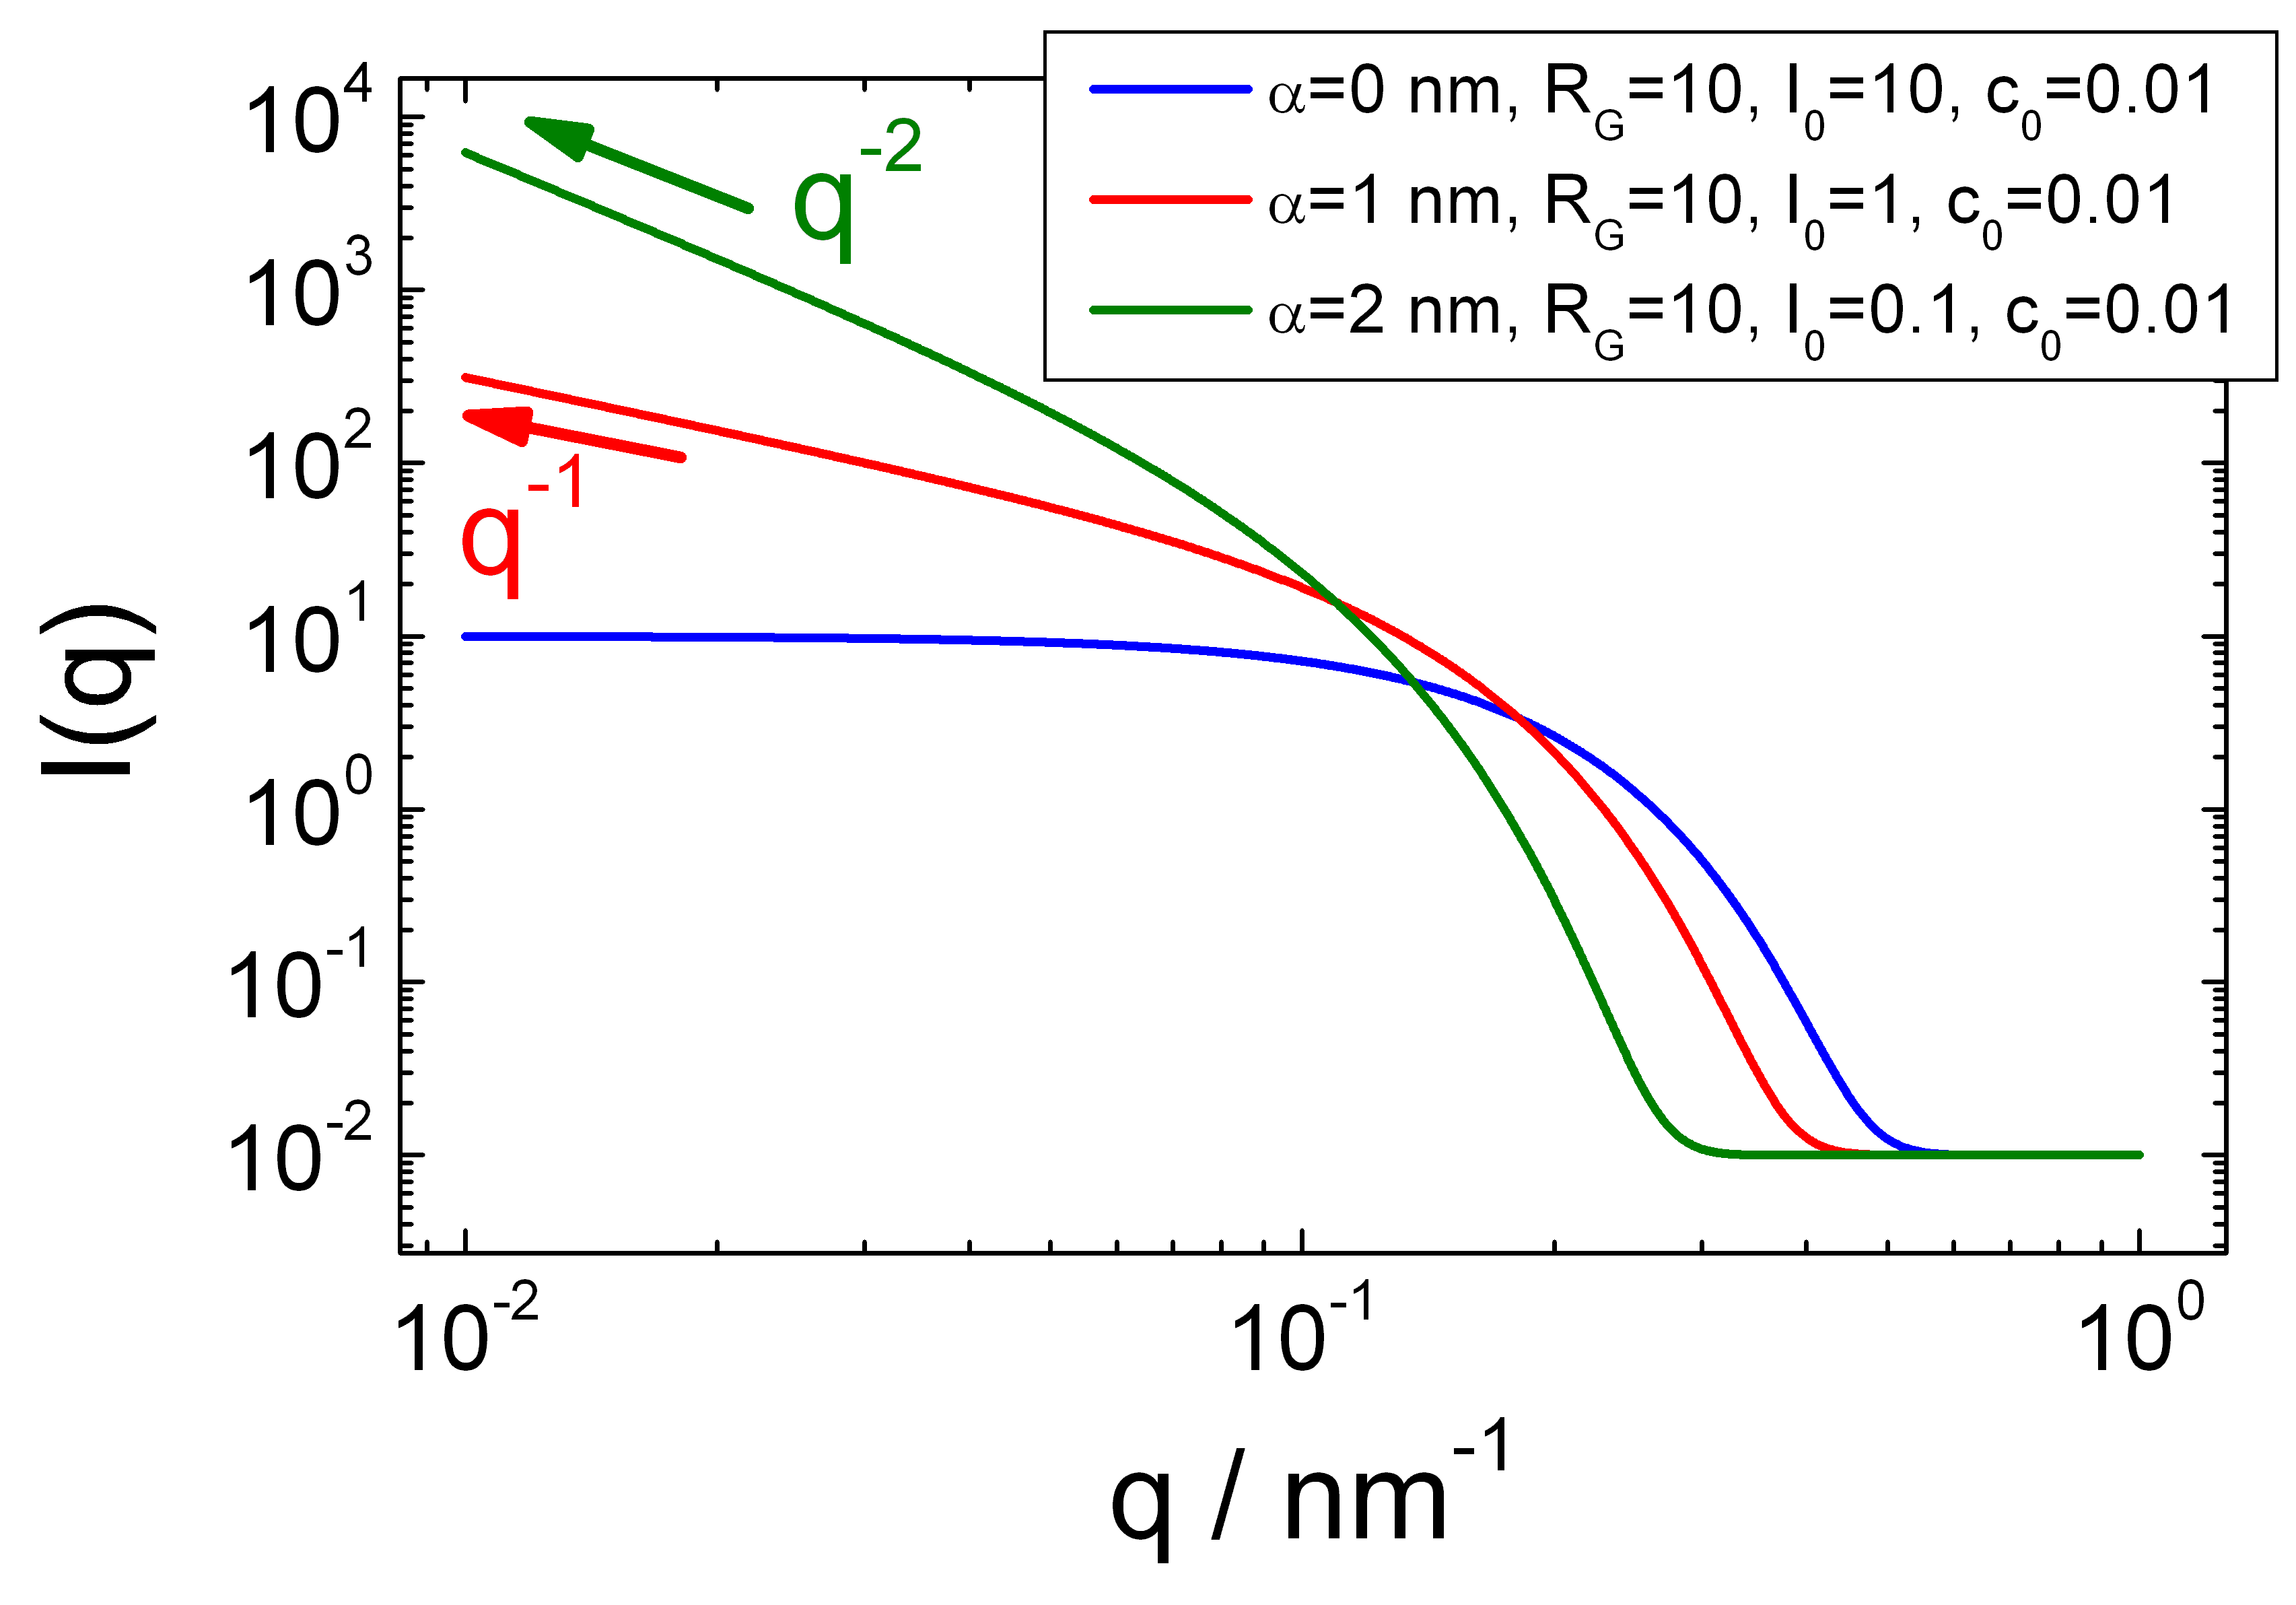
\includegraphics[width=0.85\textwidth,height=0.6\textwidth]{generalizedGuinierIq.png}
\end{center}
\caption{generalized Guinier law} \label{fig:generalizedGuinierIq}
\end{figure}
